\documentclass{article}
\usepackage{graphicx} % Required for inserting images
\usepackage[margin=2.5cm]{geometry}
\usepackage[T1]{fontenc}
\usepackage{lmodern}
\usepackage{booktabs}
\usepackage{caption}
\usepackage{float}
\usepackage[hidelinks]{hyperref}

\graphicspath{{figures/}{./}}

\title{BodySync: A Personal Stress Score from Your Wristband}
\author{Swayam Lakhotia \and Bhavya Bajaj \and Ananya Khaitan}
\date{November 2026}

\begin{document}
\maketitle

\section{The idea}

Wristbands like the Empatica record heart rate, sweat (EDA) and skin temperature all day. Sun et al.~\cite{sun2026trust} showed that these signals react when people are under pressure, but analysed each signal separately, in a single lab session. \textbf{BodySync} turns them into one 0--100 score for everyday use: 100 means your body is at \emph{its own} normal, and lower means it is reacting the way it does under stress.

Everyone's normal is different, so BodySync compares you only with yourself, never with other people.

\section{What we tried first}

Our first version asked whether the signals \emph{move together} the way they usually do (``sync''). For every 30 minutes we measured how strongly each pair of signals rises and falls together. This carried almost no information: given only sync, a model told asleep, resting and active apart 37\% of the time (random guessing: 33\%), and it did not pick out lab stress on WESAD (0.46, where 0.5 is a coin flip). How far the signals are from a person's own normal worked much better, so the final BodySync is built on that.

\section{How BodySync works}

\begin{enumerate}
\item \textbf{Your normal.} Each person's usual heart rate, sweat and temperature.
\item \textbf{Stress signals,} measured against that normal: sweat bursts (small, fast spikes in sweat, which jump from about 2 to about 10 per minute under stress), the fast and slow parts of the sweat signal, whether heart rate and temperature are rising or falling, and how much each changed over the last 10 minutes.
\item \textbf{A trained model} combines these, then adapts to each person using their own unlabelled days (self-training).
\item \textbf{The score} is smoothed over the last few minutes, since stress lasts minutes, not seconds.
\end{enumerate}

\section{Data}

\begin{table}[H]
\centering\small
\caption{Datasets. Citation counts from OpenAlex, November 2026.}
\begin{tabular}{llrrl}
\toprule
Dataset & Setting & People & Citations & Stress label \\
\midrule
ZU-PWD '25~\cite{zupwd} (ours) & daily life & 27 & -- & none (used for the demo) \\
WESAD~\cite{wesad} & lab & 15 & 1{,}352 & speech + maths test \\
Stress-Predict~\cite{stresspredict} & lab & 35 & 113 & Stroop test + interview \\
Stress + exercise~\cite{stressexercise} & lab & 36 & 37 & stress tasks + cycling \\
Nurse stress~\cite{nurse} & hospital & 15 & 119 & nurse-rated stress \\
ADARP~\cite{adarp} & daily life & 11 & 13 & button press when stressed \\
CAN-STRESS~\cite{canstress} & daily life & 62 & 1 & stress ratings 0--9 \\
AffectiveROAD~\cite{affectiveroad} (new) & real driving & 9 & 125 & city traffic vs rest \\
\bottomrule
\end{tabular}
\end{table}

All eight stress datasets use the Empatica E4, the older version of the EmbracePlus in our own dataset, which records the same signals.

\section{How we tested it}

\begin{itemize}
\item \textbf{Locked test people.} Before building the final system we set aside 40\% of the people in every dataset. All improvements were developed on the other 60\%, and the locked group was used once, at the very end. All results below are on them.
\item \textbf{Unseen people only.} Each test person is scored by a model that never saw their labels.
\item \textbf{The number.} For each person: take one stressed moment and one calm moment; how often does the stressed one score lower? 0.5 is a coin flip and 1 means always (the within-person AUC).
\item \textbf{Leak check.} With each person's stress labels scrambled, the final model scores 0.51 on average, a coin flip, so the gains are not an artefact.
\item \textbf{Shortcut checks.} In lab studies, stress can come with things that are not stress: talking and moving during the task, or always coming before the rest periods. The lab results hold with wrist movement removed from the model (WESAD 0.99+, Stress + exercise 0.91, Stress-Predict 0.88) and when rest periods right after a stressor are left out (0.99+, 0.91, 0.90). Timing is harder to rule out: in these studies stress always comes at the same point in the session, so a model given only the clock also scores high (WESAD 0.97, Stress-Predict 0.96, Stress + exercise 0.78). BodySync never sees the clock, but lab data alone cannot prove it is not partly tracking time; the driving test below does not have this problem.
\end{itemize}

\section{Results}

\begin{table}[H]
\centering\small
\caption{Locked test people: how well each version picks out stress (0.5 = coin flip, 1 = always).}
\begin{tabular}{llccc}
\toprule
Dataset & Setting & Test people & First version & Final BodySync \\
\midrule
WESAD$^*$ & lab & 6 & 0.99 & \textbf{0.99+} \\
Stress + exercise & lab & 14 & 0.60 & \textbf{0.91} \\
Stress-Predict & lab & 14 & 0.64 & \textbf{0.90} \\
CAN-STRESS & daily life & 10 & 0.61 & \textbf{0.67} \\
Nurse stress$^\dagger$ & hospital & 4 & 0.52 & 0.50 \\
ADARP$^\dagger$ & daily life & 4 & 0.53 & 0.55 \\
\midrule
Average, all six & & & 0.65 & \textbf{0.76} \\
Average, datasets with $\ge$5 test people & & & 0.71 & \textbf{0.87} \\
\bottomrule
\end{tabular}

\smallskip
\footnotesize $^*$Six test people; WESAD's speech and mental-arithmetic stressor is very strong, so even the simple first version scores 0.99. $^\dagger$Four test people: too few to judge (resampling the people, the nurse result could lie anywhere between 0.29 and 0.65).
\end{table}

\paragraph{Lab stress.} The final BodySync picks out stress about 90\% of the time or better on every lab dataset, up from about 0.6 on the two harder ones. On Stress-Predict, all 14 test people scored lower under stress.

\paragraph{Everyday life.} On CAN-STRESS, the largest daily-life dataset, BodySync improves from 0.61 to 0.67. One caution: in CAN-STRESS the calm reports cluster in the evening, so time of day may explain part of this; too few people report stress and calm at matching hours to separate the two. The nurse and ADARP results stay close to a coin flip, but with four test people each they are too small to judge either way. Everyday stress is milder than a lab stress test and is only reported a few times a day, which makes it the hard part.

\paragraph{What helped.} Every idea was tried on the development people and kept only if it helped on average. The biggest gains came from how much the signals changed over the last 10 minutes, smoothing the score, and splitting sweat into its fast and slow parts; self-training added a little. Pooling all datasets, separate normals for still and moving, other model types, a normal built only from past days, and training on exactly the tested comparison did not help. Two later rounds aimed at everyday life (learning from all everyday datasets together; scoring only while still) helped on the development people but not consistently on two further, disclosed looks at the locked people, so the final system stays as above.

\subsection*{A brand-new dataset: real driving}

After the final system was frozen we added AffectiveROAD~\cite{affectiveroad} from the MIT Media Lab: 9 drivers on 13 real drives through city traffic and on the highway, wearing the same Empatica wristband, with a 15-minute rest before and after. The dataset's own stress rating confirms that city driving is the stressful part (0.70--0.84, against about 0.5 on the highway). Nothing was tuned on it; the frozen system was run once.

\begin{table}[H]
\centering
\caption{AffectiveROAD, every driver a new test person.}
\begin{tabular}{lcc}
\toprule
Comparison & First version & Final BodySync \\
\midrule
City vs highway (both driving)$^\dagger$ & 0.73 & \textbf{0.76} \\
City driving vs resting afterwards$^\ddagger$ & 0.83 & \textbf{0.92} \\
\bottomrule
\end{tabular}

\smallskip
\footnotesize $^\dagger$Model trained only on the other datasets; the model trained on the other drivers gets 0.61 here. $^\ddagger$Model trained on the other drivers.
\end{table}

City vs highway is the fair test: both are driving, and neither wrist movement nor time since the start of the drive explains the difference (on their own they score 0.38 and 0.50); with scrambled labels it gets 0.55. City vs resting is partly just driving vs sitting still (wrist movement alone scores 0.90), even though all 9 drivers scored lower in the city. BodySync does not follow the dataset's moment-to-moment stress rating within a drive (correlation about 0.1).

\section{What a user sees}

\begin{figure}[H]
\centering
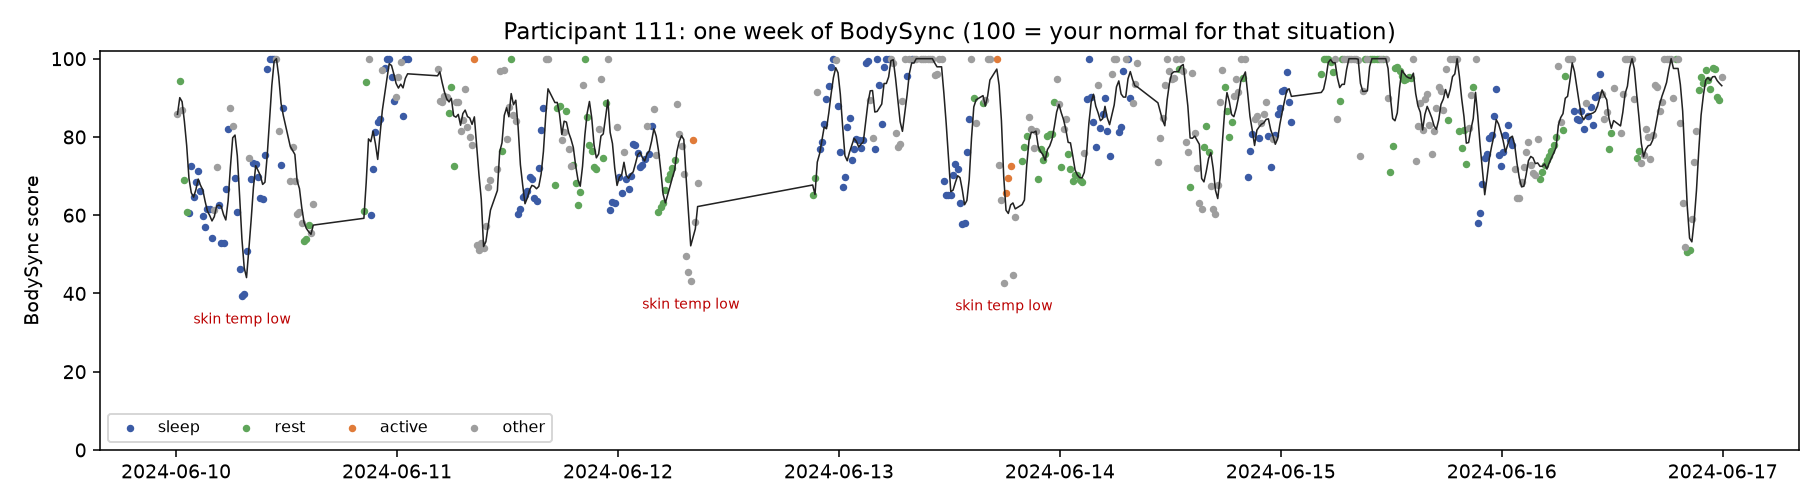
\includegraphics[width=0.9\linewidth]{fig3_example_week.png}
\caption{One week of BodySync on our own dataset (ZU-PWD): a score every 15 minutes, coloured by situation, with the reason for the lowest points. ZU-PWD only has one-minute summaries, so this uses the basic version without sweat bursts.}
\end{figure}

\section{Takeaways}

\begin{itemize}
\item Comparing your signals with your own normal works; how they move together does not.
\item On lab stress, BodySync reaches about 0.9 or better on every dataset, on people it never saw (though lab timing cannot be fully ruled out).
\item On real roads it scores 0.76 for city vs highway with a model that never saw the dataset, and movement or timing cannot explain it.
\item In daily life it improves on the largest dataset; mild, self-reported everyday stress remains the hard part.
\end{itemize}

\section{Limitations}

\begin{itemize}
\item The everyday-life datasets have few test people (4--10), so their results are uncertain.
\item Each person's normal is computed from their whole recording; a real app would build it from past data only.
\item ZU-PWD has only one-minute summaries and no stress labels, so the final model could not be tested on our own data.
\end{itemize}

Code and all results: \url{https://github.com/swaylakh/bodysync}

{\footnotesize
\begin{thebibliography}{9}
\setlength{\itemsep}{0pt}
\bibitem{sun2026trust} X.~Sun, R.~Ma, S.~Wei, P.~Cesar, J.~A.~Bosch, A.~El~Ali. Understanding trust toward human versus AI-generated health information through behavioral and physiological sensing. \emph{International Journal of Human-Computer Studies}, 209:103714, 2026.
\bibitem{zupwd} Evangelista et al. Zayed University Physiological Wellness Dataset 2025 (ZU-PWD '25). IEEE DataPort, 2025. doi:10.21227/2tth-wj12.
\bibitem{wesad} P.~Schmidt, A.~Reiss, R.~D\"urichen, C.~Marberger, K.~Van~Laerhoven. Introducing WESAD, a multimodal dataset for wearable stress and affect detection. \emph{ICMI}, 2018.
\bibitem{stresspredict} T.~Iqbal et al. Stress monitoring using wearable sensors: a pilot study and Stress-Predict dataset. \emph{Sensors}, 22(21):8135, 2022.
\bibitem{stressexercise} A.~Hongn, F.~Bosch, L.~E.~Prado, J.~M.~Ferr\'andez~Vicente, M.~P.~Bonomini. Wearable physiological signals under acute stress and exercise conditions. \emph{Scientific Data}, 12:520, 2025.
\bibitem{nurse} S.~Hosseini et al. A multimodal sensor dataset for continuous stress detection of nurses in a hospital. \emph{Scientific Data}, 9:255, 2022.
\bibitem{adarp} R.~K.~Sah et al. ADARP: a multi modal dataset for stress and alcohol relapse quantification in real life setting. \emph{IEEE BSN}, 2022.
\bibitem{canstress} R.~Rahimi~Azghan et al. CAN-STRESS: a real-world multimodal dataset for understanding cannabis use, stress, and physiological responses. \emph{IEEE BSN}, 2025.
\bibitem{affectiveroad} N.~El~Haouij, J.-M.~Poggi, S.~Sevestre-Ghalila, R.~Ghozi, M.~Ja\"idane. AffectiveROAD system and database to assess driver's attention. \emph{ACM SAC}, 2018.
\end{thebibliography}
}

\end{document}
